%\documentclass{sig-alternate-2013}
\usepackage{wrapfig}
\usepackage{balance}  % for \balance command ON LAST PAGE  (only there!)
%\usepackage{algorithmic}
%\usepackage{algorithm}
\usepackage[lined]{algorithm2e}
\usepackage{multirow}
\usepackage{subfigure}
\usepackage{graphicx}
\usepackage{caption}
\usepackage{amsmath}
\usepackage{amssymb}
\usepackage{amsfonts}
\usepackage{xspace}
\usepackage{url}
\usepackage{./tweaklist}
\usepackage[show]{./chato-notes}
\usepackage{color}
\usepackage{hyperref}

%\usepackage[T1]{fontenc}



% Paragraphs
\newcommand{\spara}[1]{\smallskip\noindent{\bf #1}}
\newcommand{\mpara}[1]{\medskip\noindent{\bf #1}}
\newcommand{\para}[1]{\noindent{\bf #1}}
\newcommand{\IGNORE}[1]{}

\newcommand{\yahoo}{{\sf Yahoo!}}

%\renewcommand{\enumhook}{\setlength{\topsep}{0.2pt}
%\setlength{\itemsep}{0pt}}

\newcommand{\alg}[1]{\bigbreak\noindent{\bf #1}}
\newcommand{\algskip}{\itemsep=-8pt\baselineskip=0pt}
\newcommand{\commentedtext}[1]{}
\newcommand{\myalgostyle}[1]  {{#1}\xspace}
%% my algorithms
\newcommand{\optselect}{\myalgostyle{OptSelect}}
%\newcommand{\optselect}{OptSelect\xspace}
\newcommand{\M}{$\mathbf{M}$}
\newtheorem{example}{Example}
\newtheorem{definition}{Definition}
\newtheorem{theorem}{Theorem}
\newtheorem{lemma}{Lemma}
%\clubpenalty=10000 
%\widowpenalty = 10000

%%%%%% Some new definitions for this report
\newcommand{\W}{\textbf{W}^t}
\newcommand{\HH}{\textbf{H}^t}
\newcommand{\G}{\textbf{G}^t}
\newcommand{\MT}{\textbf{M}^t_T}
\newcommand{\MC}{\textbf{M}^t_C}
\newcommand{\Htt}{\textbf{H}^{t-1}}
\newcommand{\Gtt}{\textbf{G}^{t-1}}
\newcommand{\X}{\textbf{X}^t}
\newcommand{\U}{\textbf{U}^t}
\newcommand{\I}{\textbf{I}}
\newcommand{\0}{\textbf{0}}
\newcommand{\e}{\textbf{e}}


\begin{document}
\permission{Permission to make digital or hard copies of all or part of this work for personal or classroom use is granted without fee provided that copies are not made or distributed for profit or commercial advantage and that copies bear this notice and the full citation on the first page. Copyrights for components of this work owned by others than ACM must be honored. Abstracting with credit is permitted. To copy otherwise, or republish, to post on servers or to redistribute to lists, requires prior specific permission and/or a fee. Request permissions from Permissions@acm.org.}
\conferenceinfo{KDD'15,}{August 10-13, 2015, Sydney, NSW, Australia.} 
\copyrightetc{\copyright~2015 ACM. ISBN \the\acmcopyr}
\crdata{978-1-4503-3664-2/15/08\ ...\$15.00.\\
DOI: http://dx.doi.org/10.1145/2783258.2783319}

\clubpenalty=10000 
\widowpenalty = 10000

%\conferenceinfo{KDD'15,} {Sydney, Australia.  Aug 10 -- 13, 2015}
%\CopyrightYear{2015}


% ****************** TITLE ****************************************
\title{Leveraging Social Context for Modeling Topic Evolution}

% ****************** AUTHORS **************************************

\numberofauthors{5}
%\author{
%\alignauthor Janani Kalyanam$^*$ 
%\alignauthor Amin Mantrach$^+$  
%\alignauthor Diego Saez-Trumper$^+$
%\and
%\alignauthor Puya Vahabi$^+$
%\alignauthor Gert Lanckriet$^*$
%}
\author{
 \alignauthor Janani Kalyanam \\
\affaddr{Univ. of California, San Diego} \email{jkalyana@ucsd.edu} \\
\alignauthor Amin Mantrach \\ 
\affaddr{Yahoo Labs\\ Barcelona, Spain} \email{amantrac@yahoo-inc.com}
\and
 \alignauthor Diego Saez-Trumper \\ 
\affaddr{Yahoo Labs \\ Barcelona, Spain}\email{dsaez-trumper@acm.org} 
\alignauthor Hossein Vahabi \\
\affaddr{Yahoo Labs \\ Barcelona, Spain} \email{puya@yahoo-inc.com}
\alignauthor Gert Lanckriet \\
\affaddr{Univ. California, San Diego} \email{gert@ece.ucsd.edu} \\
}

\maketitle \sloppy
\vspace{-1cm}
% THE ABSTRACT.
\begin{abstract}
Topic discovery and evolution (TDE) has been a problem which has gained
long standing interest in the research community.  The goal in
topic discovery is to identify groups of keywords from large corpora so that the information in those
corpora are summarized succinctly.  The nature of text corpora has changed
dramatically in the past few years with the advent of social media.  
Social media services allow users to constantly share, follow and comment
on posts from other users.  Hence, such services have given a new
dimension to the traditional text corpus.  The new dimension being that
today's corpora have a \emph{social context} embedded in them in terms of the
community of users interested in a particular post, their profiles etc.  
We wish to harness this social context that comes along with
the textual content for TDE.  In particular, our goal is to both
qualitatively and quantitatively analyze when
social context actually helps with TDE.
Methodologically, we approach the problem of TDE by a proposing non-negative matrix
factorization (NMF) based model 
that incorporates both the textual information
and social context information.  We
perform experiments on large scale real world
dataset of news articles, and use Twitter as the platform providing information
about the social context of these news articles.
We compare with and outperform
several state-of-the-art baselines. Our conclusion is that using
the social context information is most useful when
faced with topics that are particularly difficult to detect.
\vspace{-0.2cm}
%The field of topic discovery and evolution has always garnered plenty of interest
%from the research community.
%Recently, several successful algorithms modeling topic evolution have been proposed.
%However, most of them use the textual information
%to discover and model the evolution of topics.  This can often limit the kind of topics 
%being detected to only those which have a strong textual
%topical focus.
%However, in reality, as the topic evolves, the vocabulary and the focus of
%the topic may change, and relying on textual content
%alone may not solve the problem. 
%In this paper, we wish to use the social context associated with user activities
%in addition to textual content to model the evolution of topics.
%We wish to harness the social community information for detecting topics whose
%textual content may be varied, but have a strong community
%of users interested in them. We approach the problem by simultaneously modeling the evolution 
%of the social communities and the evolution of topics by using a 
%multimodal time series based non-negative matrix factorization.  The
%multimodal aspect stems from the fact that both content \emph{and} social
%context information are used to discover and model the evolution of topics.
%We perform experiments on large scale realworld dataset based on Twitter
%data.  Through experiments, we show that there is a significant improvement from
%using both content and social context information, as opposed to using 
%the content alone.
%We also show better performance when compared
%to  other state-of-the-art topic detection algorithms which include social information,
%and those which model topic evolution.
%
\end{abstract}

\category{I.5.4}{Pattern Recognition}{Applications: Text processing}
%\category{G.1.3}{Numerical Linear Algebra}{Sparse, structured, and very large systems (direct and iterative methods);}
\vspace{-0.5cm}
% INCLUDE THESE IN THE FINAL VERSION.
%\terms{Algorithms, Theory}

% INCLUDE THESE IN THE FINAL VERSION.
\keywords{Social networks, topic discovery, topic monitoring, topic tracking,
collective factorization}

% A GENERAL INTRODUCTION.
\section{Introduction}
\label{sec:introduction}
\section{Introduction}
Ebola virus disease is a communicable disease characterized by severe
symptoms (e.g. nausea, vomiting, haemorrhaging) and a very high
fatality rate \cite{WHO-Ebola-Response-Team:2014aa}.   The 2014 Ebola
outbreak --- the largest outbreak of Ebola in history --- began in
Guinea around January 2014 and rapidly spread to neighboring West
African countries (Sierra Leone, Liberia), with the World Health
Organization classifying the outbreak as a \emph{Public Health
  Emergency of International Concern} in August of that
year \cite{Weyer:2015aa}.  As of December 31st 2015, it is estimated
that there have been almost 30,000 cases associated with the outbreak,
with over 11,000 deaths\footnote{www.webcitation.org/6ePMzFc5a}.  Only 7 cases occurred outside Africa (4 in
the United States, and 1 each in Italy, the United Kingdom, and
Spain), resulting in 1 fatality in the United States.  Despite the
very low disease prevalence in the United States, public concern
regarding Ebola risk remained elevated throughout the
outbreak \cite{Towers:2015aa}.

Publicly available social media services, in particular micro-blog platforms like Twitter, are
increasingly recognized as a valuable data source for understanding
public attitudes and
opinions towards health issues, especially when combined with
computational approaches like Natural
Language Processing and Machine Learning \cite{Dredze:2012qy}.     Public attitudes towards vaccination
\cite{Salathe:2011aa}, novel tobacco products \cite{Myslin:2013aa},
illegal drugs \cite{Krauss:2015aa}, and eating disorders \cite{DBLP:conf/ehealth/Choudhury15} have all been investigated
using a combination of social media data and computational techniques.   

% Twitter, in conjunction with
% computational methods, has been used with success in
% understanding public attitudes towards vaccination
% \cite{Salathe:2011aa}, novel tobacco products \cite{Myslin:2013aa},
% and illegal drugs \cite{Krauss:2015aa}.    

In this work, 
%which builds on previous work investigating
%Ebola rumors [reference left-out for double blind review] %\cite{DBLP:journals/corr/KalyanamVDCL15},  
we used a corpus of 10.5 million Ebola-related tweets
generated in the United States during October 2014 --- the height of
the outbreak ---
%\textcolor{blue}{JANANI:  ML learning-based
%  topic modeling methods} 
to create \emph{topical timelines} that reveal 
topic progression during the outbreak by using a novel topic modeling
algorithm that explicitly models the evolution of topics
as emerging, fading, and changing.
In order to develop the
timelines, we followed a three step approach: (1) segment the data into
daily blocks, (2) apply our topic modeling algorithm to each daily
block, and (3) map and merge daily topics to create a topical
timeline (i.e. events).

An analysis of our empirically-derived Ebola timeline showed that, in terms of
their temporal duration,  identified events fell into three main groups:  \emph{long-term} events which
lasted at least 5 days,  \emph{medium-term} events which lasted between
2 and 4 days, and \emph{short-term} events which lasted for 1 day.
Generally,  long-term, enduring events tend to be those with repercussions
that might possibly put the health of the public at risk
(e.g. suspected new cases in the United States), and hence cause
anxiety in the general public.   We also observed
that any event which has a positive connotation (e.g. philanthropic
donations to help in the Ebola effort) tends to be either a
short-term or medium-term event.   Further, we discovered that a
substantial number of the  short-lived events (i.e. short-term and
medium-term events) that emerged from the data set are
memes and jokes related to Ebola.   Finally, we noted that some episodes
of public health importance (e.g. new cases) tend to generate
short-term events if these occur outside the United States,
indicating that overseas, non-US events are of limited interest to US-based
Twitter users.


 Insights gleaned from this 
Twitter-based event tracking method could be utilized by
both international public health organizations (e.g. \emph{World Health
Organization}, \emph{European Centre for Disease Prevention and Control}) and national
public health entities (e.g. United States \emph{Centers for Disease
  Control and Prevention}, \emph{Public Health Agency of Canada})  to
monitor public opinion in future outbreaks with the goal of  supporting situational 
awareness, assessing the strength and duration of public concerns, 
and identifying potential opportunities for health education.

The paper is structured as follows.  Section \ref{sec:related} describes related work;
Section \ref{sec:data_and_model} describes the data and its attributes; Section \ref{sec:timeline_generation} describes
the event timeline generation methodology, and also introduces a novel topic model
which explicitly incorporates evolving content into its framework; Section \ref{sec:comparison}
presents a quantitative evaluation of the topic model(s) used in this work;
Section \ref{sec:timeline} presents the findings and inferences of the timeline created
from Section \ref{sec:timeline_generation}.  We end with a conclusion in Section \ref{sec:conclusion}.



\section{Comparison to previous work}
\label{sec:comparison_to_previous_work}
%!TEX root = paper.tex
There are two families of work which we delve into to provide an overview of
related papers: one is the family of work on TDE, and the other is
family of work that uses some type of link structure (either derived from citation networks,
or other means) for topic modeling.  Works which fall under the latter
family tree generally do not model the evolution of topics that are discovered, and hence do not
incorporate a temporal aspect to the model they develop.  To the best of our knowledge, 
our work is the first to combine both topic discovery and evolution with link structure.
More importantly, our work is the only one which studies where the soft spot really lies.
Meaning, we comprehensively study through experiments for what kind of topics does
the social context of an article through user interactions really produce improvements in performance.

\emph{Topic discovery and evolution} has been a subject which has garnered plenty of attention for more than a decade 
but has gained renewed interest in recent 
years with the advent of the social media \cite{Sayyadi:2009,Becker:2009}.   
The most effective models developed by the topic tracking community is generally built on
some well-known topic discovery model (or topic model) with a temporal aspect added to it to accommodate for the incoming
stream of data.  This is the case with NMF (non-negative matrix factorization) \cite{Lee:Nature}
based models that connects along time the learned representations for the incoming stream of
data \cite{Blei:2006, mairal2010, Saha:2012, Vaca:2014}. In the same spirit, other works extend 
generative models like latent dirichlet allocation (LDA) \cite{blei2003}
for analyzing the evolution of topics along time \cite{AlSumait:2008, Wang:2012, Kawamae:2011, Wang:2006}. 

\emph{Social information for topic detection} has masqueraded with many names in literature.
There have been entire lines of works which use the link structure between documents to model
topics.  This link structure can be built to model a certain relationship between documents.  Examples of
information that can be modeled through link structure are common authors between documents, citation networks, etc.
Many of these models derive inspiration from classical topic modeling algorithms, and extend them
to incorporate for the new modality of information now available to them.
\cite{Erosheva:2004} proposed the Link-LDA model which extends LDA to include citation information.
It replicates the graphical model used for modeling documents and words to also model documents and
citations.  It enforces that the document's topic distribution and the document's citation distribution
to be the same.  \cite{Nallapati:2008} propose Link-PLSA-LDA as a scable LDA-type model
for topic modeling and link prediction.  Relational Topic Model (RTM) was proposed by \cite{chang2009relational}
to model link between documents as a binary random variable based on the content of the document.  They
do not consider the community information.  \cite{Rosen-Zvi:2004} propose the author-topic model to
simultaneously model the content of the topic and the interest of the author using a shared hyperparameter.  
\cite{McCallum:2007} propose the topic-author-recipient model to take into account the directionality
of the link between the documents, and models the ``who-cited-whom" information.
More recently, we have works of \cite{El-Arini:2013} which represents documents through `badges',
which are essentially descriptive terms from the users sharing the documents.  However, in our
method, we model the full authorship information as a matrix and perform collective matrix factorization.
We note that none of these methods that use the link structure or authorship information consider temporal
aspect for monitoring topics.


\vspace{-0.2cm}
\section{LEARNING FROM CONTENT AND \\SOCIAL MEDIA ACTIVITY}
\label{sec:content_and_networks}
%!TEX root = paper.tex
In this section, we explain how we formulate and optimize the problem of topic discovery and evolution
using content and social context
information.  Henceforth, we refer to our method as \textbf{LTECS}, an acronym for Learning Topic
Evolution from Content
and Social media activity.  We begin with some notation.  We assume a constant flow of documents.
Let $\mathbf{X}^t$ be a $N_d^t \times N_f$ matrix at time $t$ of $N_d^t$ documents and $N_f$ 
textual features.
The complete data matrix $\mathbf{X}$ obtained by concatenating vertically the matrices $\mathbf{X}^t$ along the time steps is considered huge and 
and practically difficult to store and handle.
The simplest approach to topic detection consists of directly learning from the global matrix $\mathbf{X}$.
However, in the real world, we are observing evolving topics and trends \cite{McCallum:2007}.
Hence, using much older data to estimate current trends may lead to wrong inference. 
Another typical strategy, consists of directly learning topics from the current batch of data while 
ignoring the trend history.  One is therefore faced with the tradeoff between past and present observations.
While recent approaches modeling topic evolution do address this tradeoff \cite{Vaca:2014, AlSumait:2008}, they rely
only on the content of the documents as their primary mode of input.
In order to consider other modalities as well (e.g. the social context associated to user activities), we introduce 
in the remainder of the section a multimodal approach to model topic evolution.
For the social context input, we have associated to each document in $\mathbf{X}^t$,
a set of users who are interested in these documents.  Let
$\mathbf{U}^t$ be a $N_d^t \times N_u$ matrix at time $t$ of $N_d^t$ documents and $N_u$ users.  Here,
$N_u$ is the total number of users in the social network.  In particular, we have $\mathbf{U}^t_{ij} = 1$ if
document-$i$ has been mentioned by user-$j$, and it is $0$ otherwise.
\vspace{-0.1cm}
\subsection{The Objective Function}
Our aim is to discover topics using both $\mathbf{X}^t$ and $\mathbf{U}^t$.  We will start with
the traditional objective function for NMF and build on it.
The goal of non-negative matrix factorization is to decompose documents in terms of the underlying
latent topics.  Let us fix the number of topics to be $k$.  We would like to decompose $\mathbf{X}^t$
so that:
\begin{equation}
	\mathbf{X}^t \approx \mathbf{W}^t\mathbf{H}^t. \label{eq:topic_decomp}
\end{equation}
Here, the $\mathbf{H}^t$ is a $k \times N_f$ topic matrix.  Each row in $\mathbf{H}^t$ represents
an underlying latent topic. If the encoding features of $\mathbf{X}^t$ are the words themselves, then each entry
in $\mathbf{H}^t$ represents how frequently a particular word appears in a topic.  The $\mathbf{W}^t$ matrix
represents how each document is decomposed in terms of the topics found in $\mathbf{H}^t$.  It \emph{explains}
each document in terms of the topics discovered in the $\mathbf{H}^t$ matrix.

For each document, in addition to the textual features, we have information about which users
are interested in these documents.  Just as in Equation \ref{eq:topic_decomp}, where we decomposed
each document in terms of the latent topics, we can think of decomposing the documents in terms of the
latent communities found in the social network.  That is, we have:
\begin{equation}
	\mathbf{U}^t \approx \mathbf{W}^t\mathbf{G}^t. \label{eq:comm_decomp}
\end{equation}
The key assumption in our formulation is that we have a common decomposition matrix $\mathbf{W}^t$ for
both equations \ref{eq:topic_decomp} and \ref{eq:comm_decomp}.  Our assumption is that a 
particular community of users will be dedicated to a particular topic.  Hence, we should be able to
decompose a document in terms of its topic \emph{or} in terms of its communities in the same way. An article
about Kim Kardashian can be thought of being decomposed as $90\%$ showbiz and $10\%$ spread across the other
topics.  Our postulation is that, there is a community of users who show keen interest in showbiz news, perhaps
a community in teenage demographics.  Hence, the same document can be equivalently decomposed in terms of 
the community as $90\%$ community interested in showbiz and $10\%$ spread across the other communities.
Equations \ref{eq:topic_decomp} and \ref{eq:comm_decomp} form the backbone of the two different parts
(namely the topic and the community part) to our objective function.  The way through which we connect
the two modalities is via the $\mathbf{W}^t$ matrix, making it common to both decompositions. 
This method is traditionally referred as \emph{collective factorization}  \cite{singh:2008}, and consists of sharing one common variable across different modalities.
The same principles have also been applied in deep learning 
(by sharing a common hidden layer across different modalities)~\cite{ngiam2011multimodal}, 
and in probabilistic modeling 
(by conditioning different observed modalities on a common hidden random variable)~\cite{Blei:2003}. 

Since we also wish to model topics' evolution over time, we make use of the topics that were
discovered in the previous time steps to help in better identifying topics
in the current influx of documents.  We decompose the current influx of documents using the topics discovered
in the previous time step as follows:
\begin{equation}
\mathbf{X}^t \approx \mathbf{W}^t\mathbf{M}_T^t\mathbf{H}^{t-1}. \label{eq:prev_topic_decomp}
\end{equation}
Here, $\mathbf{H}^{t-1}$ is a matrix of topics discovered in the previous time step.  The product
$\mathbf{M}_T^t\mathbf{H}^{t-1}$ can be thought of explaining the current topics $\mathbf{H}^t$ 
as a linear combination of the previous topics.  $\mathbf{M}_T^t$ is the \emph{topic evolution} matrix.
An $\mathbf{M}_T^{t}$ matrix close to identity (or a permuation of it) tells us that the topics have not changed 
much from the previous to current time step.  We delve into analyzing this matrix, and hence
the stabiltiy of topics (and communities) in future sections.

We also add a component of monitoring communities over time.  Similar to Equation \ref{eq:prev_topic_decomp},
we model the current set of documents with respect to the previous communities as follows:
\begin{equation}
\mathbf{X}^t \approx \mathbf{W}^t\mathbf{M}_C^t\mathbf{G}^{t-1}, \label{eq:prev_comm_decomp}
\end{equation}
where $\mathbf{M}_C^t$ is the community evolution matrix.

The crux of our loss function is formed by putting together Equations \ref{eq:topic_decomp} through
\ref{eq:prev_comm_decomp}.  Our variables are $\mathbf{W}^t$, $\mathbf{H}^t$, $\mathbf{G}^t$, 
$\mathbf{M}_T^t$ and $\mathbf{M}_C^t$.  The optimization is performed one time step after another.
Hence, $\mathbf{H}^{t-1}$ and $\mathbf{G}^{t-1}$ are \emph{known} to us by time $t$.  We decompose
our loss function into the following components,
\begin{equation}
L = \mu L_T + (1-\mu) L_C + \text{R}, \label{eq:loss_function}
\end{equation}
where $L_T$ and $L_C$ are the topic and community parts of the objective function and R encompasses the regularization terms.
We impose $l_1$ regularization on $\mathbf{W}^t$, $\mathbf{H}^t$, $\mathbf{G}^t$ and both the evolution matrices
$\mathbf{M}_T^t$ and $\mathbf{M}_C^t$ to promote sparsity.  
In order to drive the loss function more towards either topic modality or the community modality of the objective,
we use a parameter $\mu \in \big[0,1\big]$.  $\mu = 0$ places full weight on the community part and $\mu = 1$ places
full weight on the topic part.

The topic part and the community part of the
objective, and the regularization terms can be written as:
\begin{align} 
L_T &= ||\mathbf{X}^t - \mathbf{W}^t\mathbf{H}^t||_F^2 +  ||\mathbf{X}^t - \mathbf{W}^t\mathbf{M}_T^t\mathbf{H}^{t-1}||_F^2,  \\
L_C &= ||\mathbf{U}^t - \W\mathbf{G}^t||_F^2 +  ||\mathbf{U}^t - \mathbf{W}^t\mathbf{M}_C^t\mathbf{G}^{t-1}||_F^2,  \\
\text{R} &= \alpha(||\mathbf{W^t}||_1 + ||\mathbf{H}^t||_1 + ||\mathbf{G}^t||_1 + ||\mathbf{M}_T^t||_1 \nonumber \\ 
		& \qquad + ||\mathbf{M}_C^t||_1) + \lambda(||\mathbf{M}_T^t - I||_F^2 + ||\mathbf{M}_C^t - I||_F^2).
\end{align}
We add a term $\lambda||\mathbf{M}^t - \mathbf{I}||_F^2$
which, depending on the value of $\lambda \in \{0,\infty\}$ controls how much importance is placed on the past and the
present. A large value of $\lambda$ places much weight on the past and vice versa.  The role of parameters $\lambda$ and
$\mu$ are analyzed in detail in Section \ref{sec:experiments}.

\subsection{The Optimization}
We minimize the loss function $L$ as shown below:
\begin{equation}
\{\mathbf{W}^t_*, \mathbf{H}^t_*, \mathbf{G}^t_*, \mathbf{M}_{T,*}^t, \mathbf{M}_{C,*}^t\} =  \textbf{argmin } \underset{\mathbf{W}^t,\mathbf{H}^t,\mathbf{G}^t,\mathbf{M}_T^t, \mathbf{M}_C^t}  L. \label{eq:optimization}
\end{equation}
Note the variables with respect to which we optimize $L$.  Of these variables, the one that is most useful for evaluation
purposes is the matrix $\HH$.  This is a matrix of word distributions for each topic.  We compare the top-$10$ words from
each topic in $\HH$ to the top-$10$ obtained from the groundtruth.  More details about groundtruth and evaluation
are provided in Section \ref{sec:experiments}.

The optmization problem in Equation \ref{eq:optimization} is not convex in all the parameters simultaneously.  
We use multiplicative updates as
in \cite{lee_1999}.  For the loss function in Equation \ref{eq:optimization}, we derive the gradients with respect to each
variable as:
\begin{eqnarray}
\begin{split}
& \bigtriangledown_{\W}L = \W(\HH{\HH}^{T} + \G{\G}^{T} \\
		&\quad {\MT}^{T}{\Htt}^{T}\Htt\MT + {\MC}^{T}{\Gtt}^{T}\Gtt\MC) \\
	&\quad - (\X{\HH}^{T}+\X{\Htt}^{T}{\MT}^{T} + \U{\G}^{T}\\
	&\quad+\U{\Gtt}^{T}{\MC}^{T} - \alpha\e{\e}^{T}) , \label{eq:gradient_W}
\end{split} \\
\bigtriangledown_{\HH}L = {\W}^T\W\HH - ({\W}^T\X - \alpha\e{\e}^T), \\
\bigtriangledown_{\G}L = {\W}^T\W\G - ({\W}^T\U - \alpha\e{\e}^T), \\
\begin{split}
\bigtriangledown_{\MT}L = &  (\HH{\HH}^{T}){\MT}^{T}({\W}^{T}\W) + \lambda {\MT}^{T} \\
						&\quad- (\HH{\X}^{T}\W+\lambda\I - \alpha\e{\e}^{T}), \\
\end{split} \\
\begin{split}
\bigtriangledown_{\MC}L = &  (\G{\G}^{T}){\MT}^{T}({\W}^{T}\W) + \lambda {\MC}^{T} \\
						&\quad  - (\G{\U}^{T}\W+\lambda\I - \alpha\e{\e}^{T}), \\ \label{eq:gradient_MC}
\end{split}
\end{eqnarray}
where $\e = [1,1,\ldots,1].$
From the Karush Kuhn Tucker first order conditions, we have the primal feasibility as:
\vspace{-0.2cm}
\begin{equation}
\W \geq \0, \HH \geq \0, \G \geq \0, \MT \geq \0 \text{ and } \MC \geq \0,
\label{eq:primal_feasibility}
\end{equation}
the stationarity condition as $L(\W,\HH,\G,\MT,\MC) = 0$, at the minimizers, ${\W}^*, {\HH}^*, {\G}^*, {\MT}^*
{\MC}^*$, and the complementary slackness:
\begin{equation}
\begin{split}
\bigtriangledown_{\G}L \odot \G & = \mathbf{0} \text{,  } \bigtriangledown_{\HH}L \odot \HH = \mathbf{0}, \\
\bigtriangledown_{\MC}L \odot \MC &\quad = \mathbf{0} \text{,  } \bigtriangledown_{\MT}L \odot \MT = \mathbf{0}, \\
\bigtriangledown_{\W}L \odot \W & \quad = \mathbf{0}.
\label{eq:KKT}
\end{split}
\end{equation}
The update equations are derived by substituting the gradients (Equations \ref{eq:gradient_W} - \ref{eq:gradient_MC}) 
in the first order conditions (Equation \ref{eq:KKT}) as below:
\begin{align}
\begin{split}
&\W \gets \W \odot \frac{N}{D}, \text{ where } \label{eq:W_update}\\
N &= (\X{\HH}^{T}+\X{\Htt}^{T}{\MT}^{T} + \U{\G}^{T}+\U{\Gtt}^{T}{\MC}^{T} \\
	&- 2\alpha\e{\e}^{T}),\\
D &= \W(\HH{\HH}^{T} + \G{\G}^{T} + {\MT}^{T}{\Htt}^{T}\Htt\MT \\
	& + {\MC}^{T}{\Gtt}^{T}\Gtt\MC), \\ 
\end{split} \\
\HH \gets &\quad \HH \odot \frac{({\W}^{T}\X-\alpha\e{\e}^{T})}{{\W}^{T}\W\HH}, \label{eq:H_update}\\
\G \gets &\quad \G \odot \frac{({\W}^{T}\U-\alpha\e{\e}^{T})}{{\W}^{T}\W\G}, \label{eq:G_update}\\
\MT \gets &\quad \MT \odot \frac{(\Htt{\X}^{T}\W+\lambda\I - \alpha)}{(\Htt{\Htt}^{T}){\MT}^{T}({\W}^{T}\W) + \lambda {\MT}^{T}}, \label{eq:MT_update}\\
\MC \gets &\quad \MC \odot \frac{(\Gtt{\U}^{T}\W+\lambda\I - \alpha)}{(\Gtt{\Gtt}^{T}){\MC}^{T}({\W}^{T}\W) + \lambda {\MC}^{T}} \label{eq:MC_update}.
\end{align}

 \textbf{Theorem 1} \emph{The loss function $L$ in Equation  (\ref{eq:loss_function}) is non increasing under the update rules in Equations (\ref{eq:W_update}),  (\ref{eq:H_update}), (\ref{eq:G_update}), (\ref{eq:MT_update}), and (\ref{eq:MC_update}).  The loss function $L$ is invariant under these updates if and only if  $\HH$, $\G$,  $\MT$ and $\MC$ are at a stationary point of the function.} The proof for update rules on $\HH$ and $\G$ comes directly from \cite{Lee:Nature}.  For the update rules $\MT$ and $\MC$ a related formal proof is given in \cite{Vaca:2014}.  Finally, the proof for update rules on $\W$ follows from \cite{Lee:Nature}. Due to the lack of space, its proof will be provided in an extended version of the paper.
\vspace{-0.1cm}


\section{DATA SET DESCRIPTION}
\label{sec:data_set_description}
%!TEX root = paper.tex
%
\begin{algorithm}
\KwData{   $z \in \mathbb{N}_{>0}$; 
            $\mathbf{X}^{(t)}$,$\mathbf{X}^{(t+1)}$,$\dots$, $\mathbf{X}^{(t+z)}$; $\mathbf{U}^{(t)}$,$\mathbf{U}^{(t+1)}$,     
                $\dots$, $\mathbf{U}^{(t+z)}$;
            $\mathbf{T}^{(t)}$,$\mathbf{T}^{(t+1)}$,$\dots$, $\mathbf{T}^{(t+z)}$; 
            We assume that we track a set of defined hashtags so that $N_h^{(t)}  = N_h^{(t+1)} = \dots = N_h^{(t+z)}  $, 
                and in particular that all the rows of $\mathbf{T}$ matrices are equal.
  }
 \KwResult{     
            Two vectors $\textbf{v}_x$,$\textbf{v}_u$ of size $N_h^{(t)}$ containing for each hashtag 
			a stability score over the content matrix $\mathbf{X}$ and       
            user interaction matrix $\mathbf{U}$.
            
 }
 \ForAll{ $i \in {1,2,\dots,N_h}$}{
    $s_x = 0$\;
    $s_u = 0$\;
     \ForAll{ $a \in {t,t+1,\dots,t+z-1}$}{
        $s_x \mathrel{+}= cos( (\mathbf{T}^{(a)} \mathbf{X}^{(a)}){\e}^T_i , (\mathbf{T}^{(a+1)} \mathbf{X}^{(a+1)}){\e}^T_i )$\;
        $s_u \mathrel{+}= cos( (\mathbf{T}^{(a)} \mathbf{U}^{(a)}){\e}^T_i , (\mathbf{T}^{(a+1)} \mathbf{U}^{(a+1)}){\e}^T_i )$\;
     }
     $\textbf{v}_x[i] = \frac{s_x}{z}$\;
     $\textbf{v}_u[i] = \frac{s_u}{z}$\;
 }
\caption{Hashtag stability scores}
 \label{alg:hashtag_stability_scores}
\end{algorithm}
\vspace{-0.4cm}
In order to accurately answer the research questions posed in Section \ref{sec:introduction}, and evaluate
our algorithm we need a dataset where the topics persist over a period of time, 
and also has a social community that accompanies it.   
We use the public dataset which was released in 2013 \cite{YatesTrumper:2013} consisting of all the articles published from 80 international 
news sources such as CNN, BBC, Aljazeera during a period of 14 days. Each news article consists of the textual content
of the article (via \texttt{html}) and a list of all tweets which link to that article over a period 
12 hours from the article's publication. The tweets containing links 
to the news articles were also collected.  From the tweets, two features were extracted: 
the author of the tweet and the hashtags present in the tweet.  The information about the author
of the tweet was used to detect the community information.  The hashtags in the tweets
were used as the groundtruth topic of the document which the tweet linked to \cite{Tsur:2012}.\footnote{We hereby use the words topic and hashtag somewhat interchangeably.}
Most of the articles were associated to a hashtag.  We discarded the ones which did not correspond to any hashtag.  
Since we wish to \emph{track} topics over
a period of time, we consider only those hashtags that appear every day (and thereby pruning 
the number of articles even further). Moreover, to avoid data sparsity of articles, 
we keep only those hashtags that have at least five articles per day. 
After all the filtering, we end up with $33,387$ articles (from an original set of $53,784$)  associated to $384$ different hashtags.
For details about
data acquisition, refer to \cite{YatesTrumper:2013}.
\subsection{Stability of Tags}\label{subsec:hashtag_stability}
\begin{figure}
\begin{center}
    \centering
    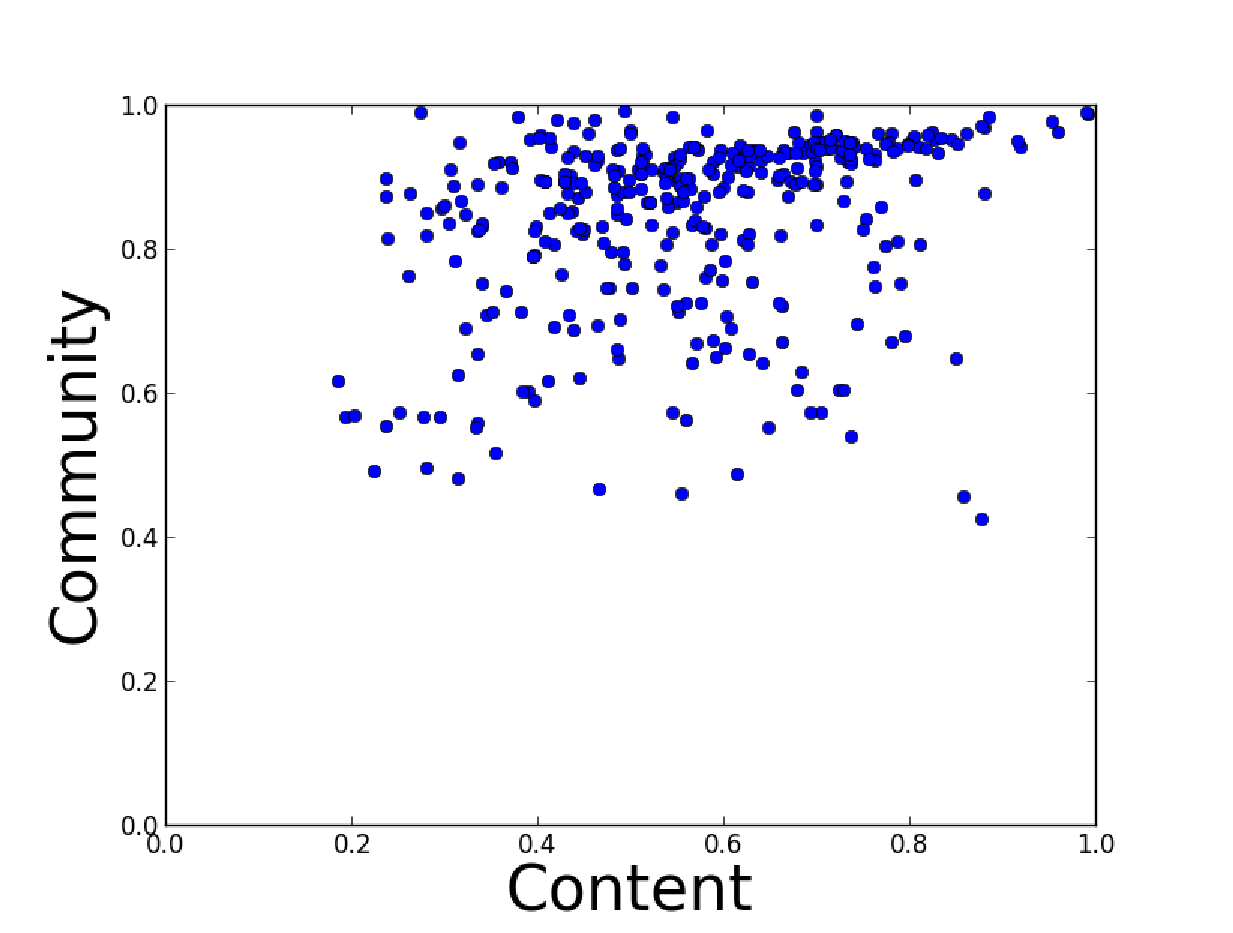
\includegraphics[width=0.5\textwidth]{KDD/images/Text-Vs-Users-sNMF-dots-new}            
\end{center}
  \caption[Stability of hashtags]{{This figure illustrates the stability of hashtags in terms of content and community information.  Each dot in the figure
is a hashtag.  The x-axis and y-axis represent content and community stability.  The content and community stability scores are 
calculated according to Algorithm \ref{alg:hashtag_stability_scores}.}  }
\label{fig:Stability}
\vspace{-0.5cm}
\end{figure}
\begin{table}
\begin{center}
\begin{minipage}[b]{1\linewidth}
{\tiny
\begin{tabular}{|lclclc|}
\multicolumn{6}{c}{\small{Twitter News Dataset}} \cr
\multicolumn{2}{c}{\bf Text-Stable} & \multicolumn{2}{c}{\bf Community-Stable} & \multicolumn{2}{c}{\bf Mixed} \cr
\#birdflu &  & \#facts &  & \#egitto3000 & \cr
\#h7n9 &  & \#celeb &  & \#hindi &  \cr
\#google &  & \#nyt &  & \#tahrir & \cr
\#football &  & \#gossip &  & \#alarabiya &  \cr
\#taxes & & \#followfriday & & \#vrwc &  \cr
\#bangladesh & & \#cbs &  & \#jan25 &  \cr
\#chinese &  & \#businessangel & & \#news &  \cr
\#climatechange &  & \#aje &  & \#rwnjalert &  \cr
\#climate &  & \#fem2 &  & \#bigtweet &  \cr
\#nkorea &  & \#opanews &  & \#business &  \cr
\#immigration &  & \#tf &  & \#india &  \cr
\#iran &  & \#interesting &  & \#smallbusiness & \cr
\#gun &  & \#top & & \#nhl &  \cr
\#lgbt &  & \#cincinnati &  & \#forbes &  \cr
\#dprk &  & \#thn24en & & \#buisnessguide &  \cr
\#nba &  & \#ihatetimwaterman &  & \#tcot &  \cr
\#japan &  & \#stopoccopywaste &  & \#financenews &  \cr
\#tax &  & \#divalishdesigns &  & \#adityaramadana & \cr
\#nuclear & & \#informate &  & \#shubhamconsultants & \cr
\#education & & \#olympic &  & \#money &  \cr
\end{tabular}
} %tiny
\centering 
\end{minipage}
\caption[A list of the top hashtags in each category.]{{This table lists the top-$20$ hashtags found in the content stable, community stable and mixed stable categories.
Basically these are closest $20$ points by Euclidean distance from $(1,0)$, $(0,1)$ and $(1,1)$ in Figure \ref{fig:Stability}
for content stable, community stable, and mixed stable hashtags respectively.  These were used as the groundtruth
for evaluating topic discovery (more details on evaluation in Section \ref{sec:experiments}).}}
\label{tab:tags}
\end{center}
\vspace{-0.8cm}
\end{table}

Recall that we use the hashtags as the groundtruth
topic of the text document.
Keeping in mind our research questions from Section \ref{sec:introduction}, we wanted to detect the three different
categories of hashtags for each dataset.
The first category of hashtags are those that are stable in terms of content, but relatively unstable in terms of community; 
meaning that the content corresponding to these hashtags does not evolve much over the period of interest, but the community
of users who tweet about these hashtags evolves quite a bit.
We call this set \emph{content stable} hashtags.  These are the supposedly `easier' topics where one may expect
that the presence of community may not particularly help in better topic discovery.
The second category of hashtags are those that are stable in terms of their community, but the content evolves a lot;
meaning that the community of users that show an interest on these tags stays relatively unchanged over a period of time,
but the actual content (in terms of vocabulary) changes a lot.
We call this set \emph{community-stable} hashtags.  These are the supposedly more difficult topics where using
the content alone may yield only poor performance, since by definition the content is not very stable.
The third category of hashtags are those that are stable in terms of both content and community, called \emph{mixed-stable}
hashtags.  
Intuitively, we posit that our model would work particularly well in discovering and monitoring those topics which 
have a stable community of active users over the period
of interest, but have a content which is evolving a lot (these are community-stable hashtags).

Following the notation specified in Section \ref{sec:content_and_networks}, we explain how we determine the 
tags which fall into the content-stable, community-stable, and mixed-stable categories.
Let us consider matrix $\mathbf{T}^{(t)}$ of size $N_h^{(t)} \times N_d^{(t)}$, 
where  $N_h^{(t)}$ is the number of hashtags produced at time $t$ and 
$N_d^{(t)}$ is the number of documents arriving at time $t$.
In particular, $\mathbf{T}^{(t)}(i,j) = 1$ if the document $j$ has been mentioned in a tweet
that contains the hashtag $i$, and $0$ otherwise.  Algorithm \ref{alg:hashtag_stability_scores} explains
how we compute a stability score for each hashtag in terms of their content and community. The essence of Algorithm
\ref{alg:hashtag_stability_scores} is as follows: by simply averaging all the documents belonging to a particular
hashtag, we obtain a representation for each hashtag in terms of features extracted from the documents. Following this procedure, each hashtag can consists of a (centroid) vector of  $N_f$ entries (i.e., in a bag-of-words representation).  We compare this representation with a similar
representation obtained for the same hashtag at the next time step using cosine similarity.  We then average
all the similarities obtained across the consecutive time steps for each hashtag.

Refer to Figure \ref{fig:Stability}.  Note that, in such a figure, the point $(1,0)$ represents perfect content stability, and zero community
stability.  To determine the set of hashtags that belong to the \emph{content stable} set, we calculate the Euclidean distance between
$(1,0)$ and all the other hashtags, and rank them in the increasing order of their distances.  Likewise for \emph{community stable} and
\emph{mixed stable} sets (using respectively the Euclidean distances to points $(0,1)$ and $(1,1)$).  
Some examples of content stable hashtags are \texttt{\#football} and \texttt{\#h7n9}; community stable hashtags,
\texttt{\#celeb} and \texttt{\#gossip} and mixed stable hashtags \texttt{\#alarabiya} and \texttt{\#forbes}.
\vspace{-0.2cm}


% EXPERIMENTS
\section{Experiments}
\label{sec:experiments}
%!TEX root = paper.
\begin{figure*}[!t]
\begin{minipage}{0.310\linewidth}
  \centering
  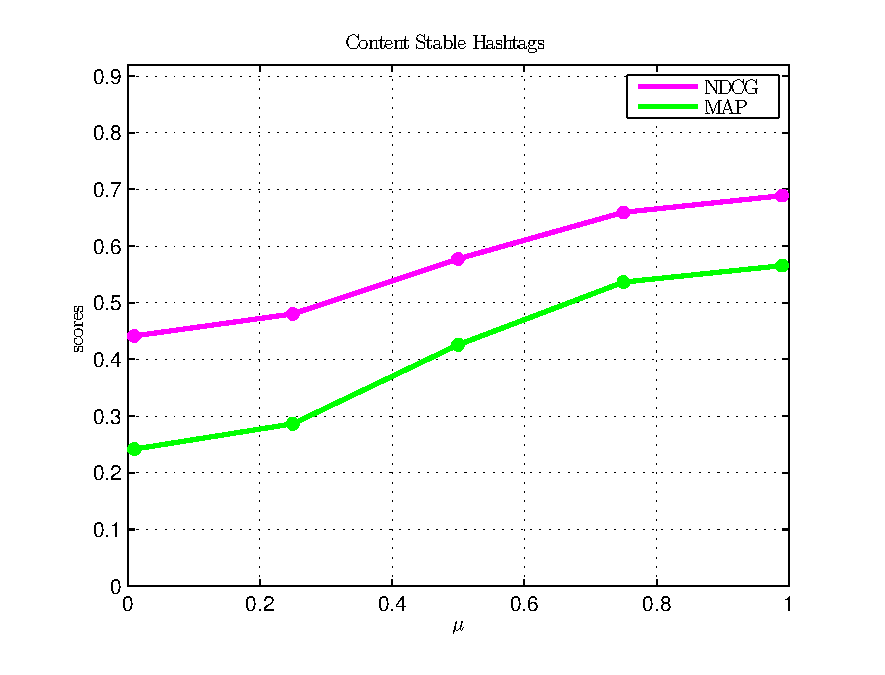
\includegraphics[width=1\textwidth]{KDD/images/content}             
   (a) content stable; $k = 5$ 
\end{minipage}
\begin{minipage}{0.310\linewidth}
  \centering
  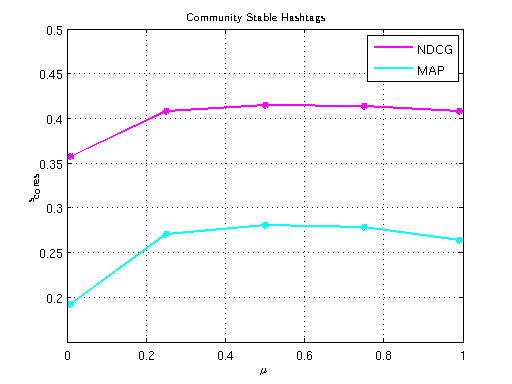
\includegraphics[width=1\textwidth]{KDD/images/community}             
  (b) community stable; $k = 5$
\end{minipage}
\begin{minipage}{0.310\linewidth}
  \centering
  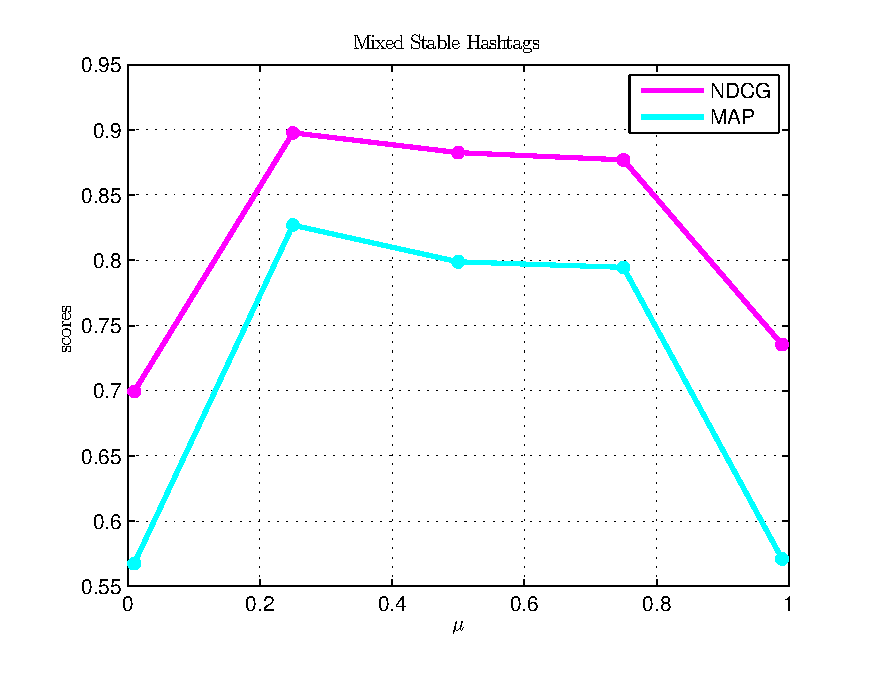
\includegraphics[width=1\textwidth]{KDD/images/mixed}             
  (c) mixed stable; $k = 5$
\end{minipage} \\
\begin{minipage}{0.310\linewidth}
  \centering
  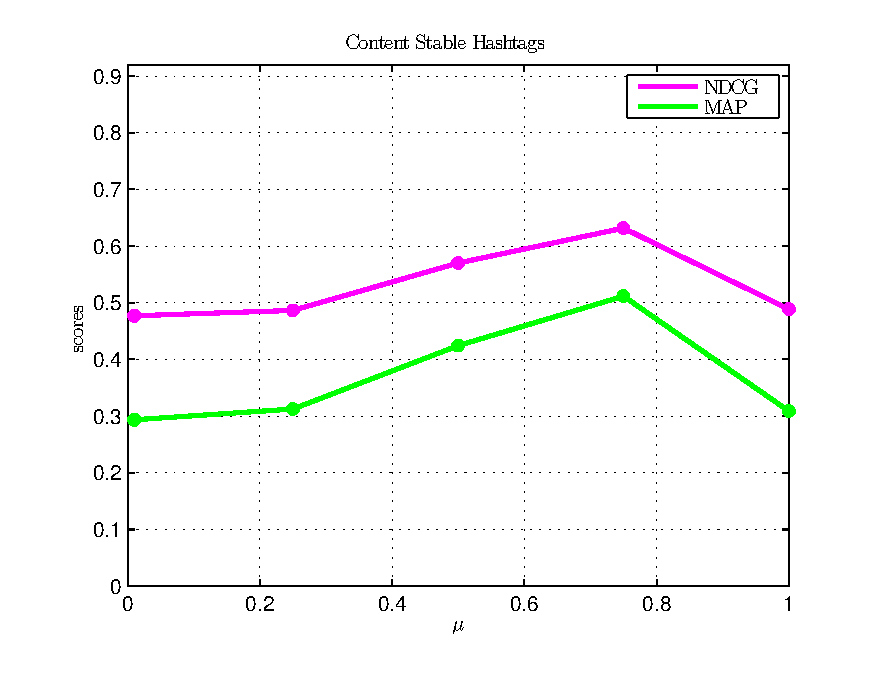
\includegraphics[width=1\textwidth]{KDD/images/content_t_15}             
   (d) content stable; $k = 15$
\end{minipage}
\begin{minipage}{0.310\linewidth}
  \centering
  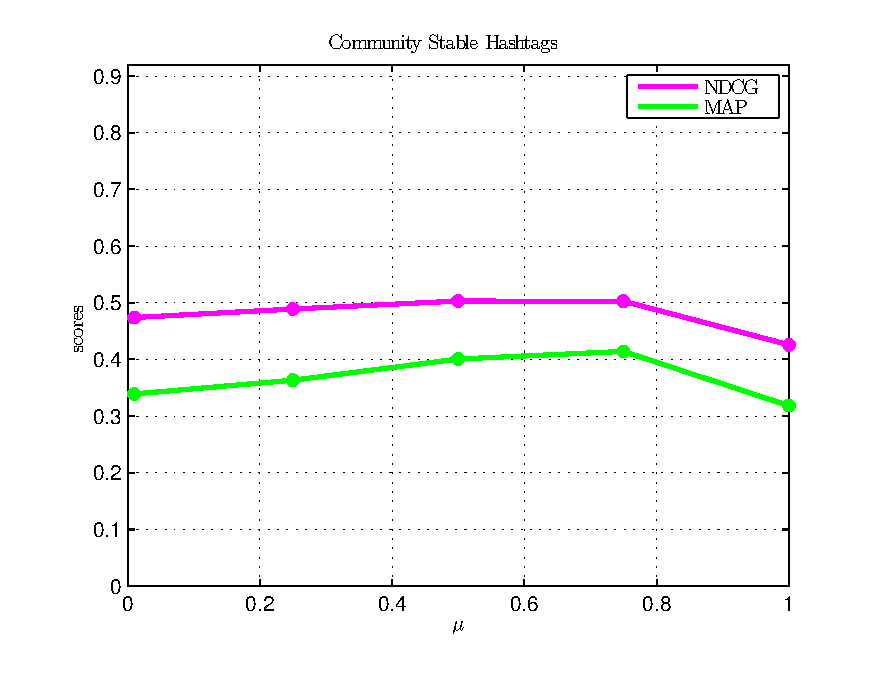
\includegraphics[width=1\textwidth]{KDD/images/community_t_15}             
  (e) community stable; $k = 15$
\end{minipage}
\begin{minipage}{0.310\linewidth}
  \centering
  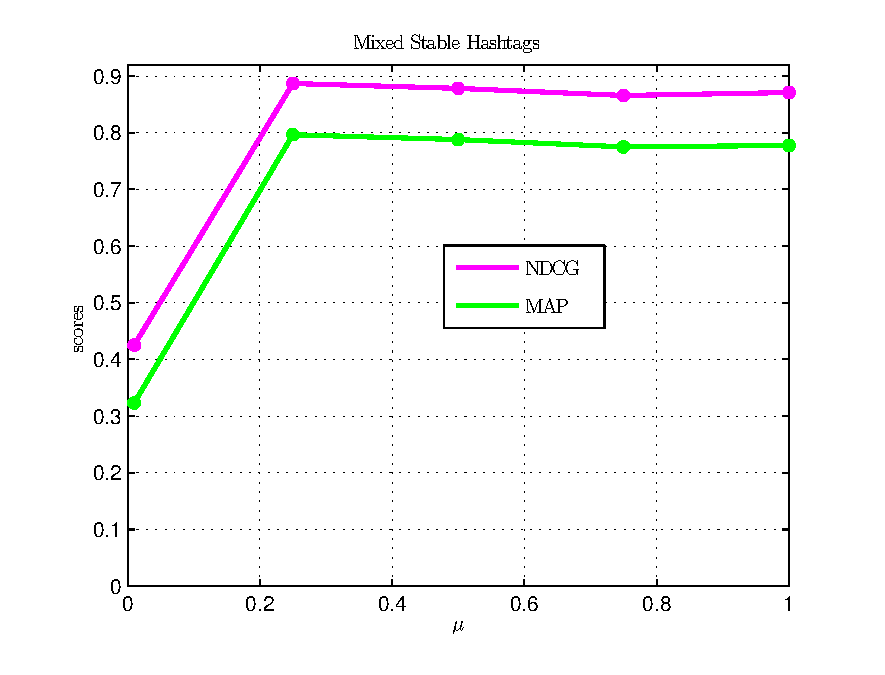
\includegraphics[width=1\textwidth]{KDD/images/mixed_t_15}             
  (f) mixed stable; $k = 15$
\end{minipage}
  \caption[Effect of $\mu$.]{{This figure illustrates the effect of the importance parameter, $\mu$ on the performance.  
Refer to Equation \ref{eq:loss_function}.  A high value of $\mu$ places more weight on the topic part of the objective
and less weight on the community part of the objective, and vice versa.
}}
\label{fig:mu_analysis}
\end{figure*}
Recall that our goal in this work is to gain a better understanding of when the
social context surrounding the documents actually improve topic discovery.
Hence, in this section, our primary focus is to provide a quantitative and 
qualitative answers to each of the research questions posed in the introduction. 
Section \ref{subsec:baselines} provides an overview about the baseline algorithms,
details how we implement them, and how we use them in our
problem setting.  Section \ref{subsec:ground_truth_evaluation}
provides details about how the groundtruth topics are obtained.  In addition,
it also explains how the topics detected by our algorithm and each of the baselines are compared with
the groundtruth  topics, and what metrics are used for the evaluations.
Then, each of the subsequent subsections are dedicated to answering one or more 
research questions.
\subsection{Baselines}
\label{subsec:baselines}
We evaluate our algorithm with several baselines.  Our baselines can be divided into two categories;
one which focuses on modeling topic evolution, and another which aims to incorporate link information
into topic modeling.

\emph{Link-PLSA-LDA} \cite{Nallapati:2008} is an algorithm which uses both the content
and link information (but does not have a temporal aspect incorporated in it). 
The link structure is built from the citation network of the documents.
The algorithm combines LDA and PLSA into a single
framework and in addition, models the topical relationship between the citing document
and the cited document.\footnote{While we do not explicitly compare to \cite{Erosheva:2004}, the
authors of Link-PLSA-LDA compare
their own work to former and claim better performance.}  The inference is carried out by
employing mean-variation approximation of the latent variables.  To implement this algorithm, 
we used the code developed by the authors which is available publicly.\footnote{\hyperref[]{https://sites.google.com/site/rameshnallapati/software}}  As input, the algorithm requires
a list of documents in a bag-of-words format, and a matrix of links between the documents.  Producing
bag-of-words for each document is straightforward.  For the link information, 
we assume that a link exists between two articles if they have a common user sharing or posting
the article.  This information was essentially derived from the $\mathbf{U}$ matrix in Section
\ref{sec:data_set_description}.  Each fresh inflow of documents is considered as a separate problem
as the model was not developed to connect topics temporally.

\emph{Collective Matrix Factorixation} (CMF) \cite{Saveski:2014, Ding:2014} 
Broadly speaking, the concept of collective matrix factorization has been
used in several applications including recommendation systems, producing hashing functions for images, co-clustering etc.
In this scenario, we will use CMF to incorporate both the social and textual aspect
of the objective in Equation \ref{eq:loss_function} but not its temporal aspect.
We compare our method to this
baseline to show that using the temporal information of tracking the textual content and community helps improve
performance.

\emph{Online-LDA} \cite{AlSumait:2008} is an algorithm which monitors topic evolution, in that it utilizes 
the information about topics detected in the previous time steps, but does not accommodate 
for the link structure between the documents.  We implemented Online-LDA based
on the original LDA code developed by David Blei\footnote{\hyperref[]{http://www.cs.princeton.edu/~blei/lda-c/}} 
(as suggested by the authors of \cite{AlSumait:2008}).  The authors
of \cite{AlSumait:2008} had found that using the topics detected in the previous time step produced the most improvement in
performance, and suggested that using the topics from earlier time steps produced only marginal improvements.  
We tested this baseline in a similar setting as well and used only the topics in the previous timestep to discover current topics.
In essense, implementing Online-LDA boils down to setting the prior on the topics according to the topic
distribution discovered in the previous time step.

\emph{Joint Past Present Decomposition} (JPP) \cite{Vaca:2014} models also the topic evolution, but as Online-LDA, is blind to the social context surrounding the  input documents.  Our method, LTECS, reduces to JPP when $\mu = 1$.
We used the code provided by the authors.\footnote{\hyperref[]{https://github.com/amantrac/TopicDiscoveryJPP}}
\subsection{Evaluation, Groundtruth and Experimental Setup}
\label{subsec:ground_truth_evaluation}
We evaluate all the algorithms by comparing a ranking of the top-$10$ words obtained by each
algorithm, and a ranking of the top-$10$ words obtained by the groundtruth.  It has been shown that
the group of top-$10$ words indeed give us a good insight about the topic \cite{sekiguchi:2006,newman2010automatic}.
All the algorithms considered here including the baselines and LTECS
discover topics by directly producing a distribution over words. 
In terms of mapping the discovered topics to the groundtruth topics, we calculated
the cosine similarity between each of the discovered topics and the groundtruth topics.
Each discovered topic was then mapped to the most similar groundtruth topic.
We borrow this procedure procedure from other state of the art experiments
in topic evolution \cite{Saha:2012}.
The distributions produced in each case are discrete and can be used 
to pick the top-$10$ words in each topic and to produce a ranking.

We now delve a bit more into how the groundtruth is obtained.  On Twitter, hashtags are a sequence of non-whitespace
characters which follow the \# sign.  It is popular convention on Twitter to embed a hashtag
in a tweet to give it context.
And as in several studies in the past, this context is used as the groundtruth topic annotations for
the news articles whose links are embedded in the tweet \cite{Tsur:2012}. 
The hashtags for each of the three categories, content stable,
community stable, and mixed stable were identified as explained in Section \ref{subsec:hashtag_stability}.

The way we calculate
the actual groundtruth topic distribution is that, 
at each time step, the $\mathbf{T}^{(t)}$
matrix (refer to Section \ref{sec:data_set_description} for notation) is premultiplied by $\mathbf{X}^{(t)}$
to obtain a resulting matrix of raw word counts for each topic.  Premultiplication of $\mathbf{T}^{(t)}$
by $\mathbf{X}^{(t)}$ basically yields the average word distribution within each hashtag.  
Once this is obtained, the highest weighted $10$ words form our groundtruth ranking.  We use
Normalized Cumulative Discounted Gain (NDCG) metric, and the Mean Average Precision (MAP) metric
to compare the rankings obtained by each algorithm to the groundtruth.  We have performed
experiments by considering the best $5,10,15 \text{ and } 20$ topics for each category.  

We now give details about the experimental setup.  Our objective function is optimized
iteratively using the multiplicative update equations (Equations \ref{eq:W_update} - \ref{eq:MC_update})
in Section \ref{sec:content_and_networks}.  The variables $\W, \HH, \G, \MT, \MC$ were given
a random non-negative initialization.  The parameters were tuned on all
the data.  In both datasets, the data spans for 14 days, and hence the topic discovery results that
we obtained are averages of the results obtained over that time period.
The $l1$ normalization parameter for CMF, the JPP model and the LTECS model were set to $0.05$.
The $\lambda$ parameter was tuned for values of $\{10, 100, 10^3 \ldots 10^7\}$.  It was consistently
observed that the algorithm yielded good performance for $\lambda = 10^7$
\footnote{While it so happens that this value of lambda worked well for the Twitter dataset, it may
not hold for other datasets.  As a matter of fact, we explore this more in Section \ref{subsec:learning_stability}
where we try to assess the quality of topics by setting $\alpha = 0.5$ and $\lambda = 0$.}.
We tuned for different values of $\mu \in \{0.01, 0.25, 0.5, 0.75, 1\}$ and picked the one which gives the best performance.
We delve more into the analysis for $\mu$ in subsequent sections.  For the baselines, all the parameters
were tuned and set internally.
\subsection{Social Information Vs Textual Content: the Trade-off}
\label{subsec:parameter_analysis}
The $\mu$ parameter from Equation \ref{eq:loss_function} allows to
bias the objective function more
towards one of the modalities, if so desired.  A high value of $\mu$ biases importance to the content part of
the objective and vice versa.  In fact, LTECS reduces to JPP when $\mu = 1$ and hence JPP can never
outperform LTECS.  This section delves into investigating how the trade-off between using content and social information
actually functions on both datasets. 

For the case of \emph{community stable} hashtags, the best performances
were achieved for $0.01 \leq \mu \leq 0.5$ (Table \ref{tab:topic_discovery_evaluation}).
This implies that when a lot of importance was placed on the social context part
of the objective, better were the topics that were detected. Refer to Figure \ref{fig:mu_analysis}b
and \ref{fig:mu_analysis}e.  These figures illustrate how the performance varies as the value of $\mu$
moves from $0$ to $1$.  Note that highest performance is achieved when $\mu \leq 0.5$.

While considering \emph{content stable} hashtags, we will focus on LTECS and JPP
in Table \ref{tab:topic_discovery_evaluation}. For $k = 5 \text{ and } 10$, we observe best
performances by \emph{both} JPP and LTECS method.  In other words, LTECS
algorithm exhibited best performance when the objective contained only the content part with $\mu = 1$.  
This suggests that for topics which have a highly focused text, we need to place all the 
importance on content.  What is more interesting is that, it implies that even if we add a little
bit of the social context information to the objective, it actually \emph{hurts} performance.
Let us contrast this result to what happens when $k = 15 \text{ and } 20$.
In those scenarios, we observe that the best performance was
obtained by LTECS, when $\mu$ was $0.75$.  
For the purest $5$ and $10$ topics, it could be that the content of those documents 
were very well defined that the usage of side information actually detracted the objective 
from the correct path.  However as the number of topics
increases ($k = 15, 20$), there is perhaps more noise in the topics and
we find that the use of community information indeed helps.  
This suggests that for the best performance one needs to know the accurate
operating spot of the $\mu$ parameter.  
The important message from analyzing the $\mu$ trade-off for content stable and community
stable hashtags is that, with very focused text, just using the content suffices. This is likely to be the case for the dominant topics (i.e. $k<10$ in our study).
On the other hand, if the text is a little noisy, the social context greatly
helps in discovering better topics. 
This is likely to be the case when tracking more than just the top dominant topics ($k>10$ in our case).  
As we argue in the introduction, in today's world,
the text is more often than not quite noisy as topics are prone to being volatile and evolving
very quickly.  Refer to Figures \ref{fig:mu_analysis}(a) and \ref{fig:mu_analysis}(d).  The figure
illustrates that the best performance is acheived when $\mu \geq 0.5$.

By definition \emph{mixed stable} hashtags have both stable content and stable communities.  
As it turns out, the best performance for LTECS is obtained when $0.25 \leq \mu \leq 0.75$.
This suggests that when we have topics which have both stable content and community,
it is necessary to give importance to both aspects.  In addition, biasing only on content
does not yield the best performance.  In Figures \ref{fig:mu_analysis}(c) and \ref{fig:mu_analysis}(f),
the best performance is achieved in the midregion of the plot.
\subsection{Comparison with the state-of-the-art}
\label{subsec:topic_discovery_experiments}
In this section, we discuss how our algorithm performs in 
comparison to state of the art baselines introduced in Section \ref{subsec:baselines}.
One of the main conclusions from analyzing the results is that, using the community
information certainly helps with better topic tracking.  This is a direct observation
from Table \ref{tab:topic_discovery_evaluation} that the NDCG and MAP values for LTECS
is higher, or at least as good as its competitors in most scenarios.  The rest of this section
will highlight where the sweet spot of the trade off between content and community
lies, and why.

For \emph{community stable topics}, as expected, good improvements were seen in the community stable hashtags.  In these hashtags,
LTECS algorithm consistently outperforms all the baselines.  It is clear that
the use of community information helps in better topic discovery.  It is also interesting
to note that the algorithm that exhibits second best performance is Link-PLSA-LDA.  
Hence, not learning from older topics does not particularly hurt Link-PLSA-LDA
in its performance when compared to Online-LDA and JPP.  This means that, for community stable topics, 
the algorithms that use some form
of social context information or link information perform better than those that discover topics using
content alone.

In the case of \emph{content stable topics}, one may expect the baselines which focus only
on the content of the documents to exhibit best performance.  This is partially true.  For $k = 5,10$,
JPP and LTECS outperform Link-PLSA-LDA and Online-LDA.  Note that in both cases
LTECS achieves the best performance only when $\mu = 1$ implying that adding community information
does not help.  On the other hand, for $k = 15 \text{ and } 20$, LTECS achieves best performance
over all the baselines.  In these cases note that the value for $\mu = 0.75$.  This implies
that adding the community information actually helps.  We already discussed this behavior in Section \ref{subsec:parameter_analysis}.
 Another thing to note here is that Link-PLSA-LDA some what consistently ranks last.  This is because
Link-PLSA-LDA, unlike LTECS lacks the tuning parameter $\mu$ which can seamlessly shift the focus of the
objective between topic and community.  It perhaps places equal weight on both, and hence fails to
make the appropriate tradeoff.

For \emph{mixed stable hashtags}, the performance is in generally very good for all the hashtags.
This becomes clear when we compare the performance metrics of content stable and community stable to mixed stable.  There
is a noticeable jump in the average NDCG and MAP scores.  This implies that, if a hashtag
has both well focused content, and a dedicated community of users, detecting those topics
are much easier. 
\begin{table*}[!t]
\begin{center}
{\small 
{\renewcommand{\arraystretch}{0.91}
\begin{tabular}{||c|c|c|cccc||}
\hline
 Category of Topic &Metric & Model & k = 5 & k = 10 & k = 15 & k = 20\\
\hline
 		    & & LTECS & 0.4081 & \textbf{0.4800} & \textbf{0.5029} & 0.5129\\
Community 	& &  & $\mu =  0.01$  & $\mu = 0.5$ & $\mu =  0.5 $ & $\mu = 0.5$\\ \cline{4-7}	
		    & NDCG & JPP & 0.3699 & 0.4496 & 0.4608 &0.4138\\
			&  & Online-LDA & 0.3903 & 0.4138 &0.4446  & 0.5667 \\
Stable       & & Link-PLSA-LDA &0.3943 & 0.4608 & 0.4761 & 0.4925\\ 
        & & CMF & 0.3454 & 0.4338 & 0.4771 & 0.4827 \\ \cline{4-7}
		& & LTECS & 0.2653 & 0.3637 & \textbf{0.4007} & \textbf{0.4173}  \\
		& &  &$\mu = 0.01$ & $\mu = 0.5 $ & $\mu = 0.5$  & $\mu = 0.5$ \\ \cline{4-7}
Hashtags&MAP & JPP &  0.2191 & 0.3596 & 0.3462 & 0.3420 \\
		& & Online-LDA & 0.2628  & 0.3160 & 0.3489 & 0.3835 \\
		& & Link-PLSA-LDA & 0.2704 & 0.3364  & 0.3658 & 0.3937 \\
        & & CMF & 0.2044 & 0.3190 & 0.3757 & 0.3665 \\
\hline
		& & LTECS &\ 0.6888 & 0.6055& \textbf{0.6317}& \textbf{0.6623} \\
Content   & &  & $\mu =  1$  & $\mu = 1$ & $\mu =  0.75 $ & $\mu = 0.75$\\ \cline{4-7}
		&NDCG & JPP & 0.6888 & 0.6055 &  0.4885&  0.6504 \\
		& & Online-LDA & 0.6815& 0.5988 & 0.6166 & 0.6684  \\
Stable  & & Link-PLSA-LDA & 0.6574 & 0.5862 & 0.6087& 0.6401\\ 
        & & CMF & 0.5846 & 0.4919 & 0.4455 & 0.4327 \\\cline{2-7}
		& & LTECS & \textbf{0.5655} &  \textbf{0.4784}& \textbf{0.5115} & \textbf{0.5559}  \\
		& &  & $\mu =  1$  & $\mu = 1$ & $\mu =  0.75$ & $\mu = 0.75$\\ \cline{4-7}
Hashtags &MAP & JPP &  0.5655 & 0.4784 & 0.3089 & 0.5411  \\
		& & Online-LDA &  0.5175 & 0.4083 & 0.4555 & 0.5443 \\
		& & Link-PLSA-LDA & 0.4890 & 0.3817  &0.4434 &0.5053  \\
        & & CMF & 0.4423 & 0.3207 & 0.2556 & 0.2557 \\
\hline
	    & & LTECS & 0.9005 & 0.8868& \textbf{0.9249}& 0.9089 \\
Mixed   & &  & $\mu =  0.25$  & $\mu = 0.75$ & $\mu =  0.25 $ & $\mu = 0.25$ \\ \cline{4-7}
		&NDCG & JPP & 0.8771 & 0.8762 & 0.4251 & 0.4580 \\ 
	    & & Online-LDA &\textbf{0.9564} & 0.9168 & 0.9111 & 0.5967 \\
Stable  & & Link-PLSA-LDA & 0.8944 & 0.9159 &0.8392 & 0.8975 \\ 
        & & CMF & 0.6712 & 0.8768 & 0.8905 & 0.8753 \\ \cline{2-7}
		& & LTECS & 0.7783 &0.7965  & \textbf{0.8964} & 0.8845 \\
		& &  & $\mu =  0.25$  & $\mu = 0.75$ & $\mu =  0.5$ & $\mu = 0.25$ \\ \cline{4-7}
Hashtags&MAP & JPP &  0.7762 & 0. 7783 & 0.3232 & 0.3644  \\ 
		& & Online-LDA & \textbf{0.9208}  & \textbf{0.8804} & 0.8841 & 0.4308 \\
		& & Link-PLSA-LDA & 0.8787 & 0.8379  & 0.7452 & \textbf{0.8982} \\
        & & CMF & 0.5329 & 0.8223 & 0.8499 & 0.8337 \\
\hline
\end{tabular}
}
}
\caption[Evaluation of topic discovery]{{Topic discovery evaluation using Normalized Cumulative Discounted Gain and Mean Average Precision metrics
for all three categories of hashtags.  $k$ stands for the number of topics.  $\lambda$ was set to $10^7$, and $\alpha$ was set to 0.05 for LTECS model.
All the values in bold represent significant improvement in performance (using Student-t test, $p < 0.05$).}}
\label{tab:topic_discovery_evaluation}
\end{center}
\end{table*}
\subsection{Learning Stability of Topics}
\label{subsec:learning_stability}
In this section, we investigate to what extent can our algorithm learn the type of
topics present in the documents; i.e., are the documents more content stable,
community stable or mixed stable. And we certainly do not want to be able to bias the
objective function more towards one of the modalities.  Hence, for all experiments
in this section, we set $\mu = 0.5$.
Recall that our loss function (Equation \ref{eq:loss_function}) is built such
that $\HH \approx \mathbf{M} \Htt$. 
The proposed model encourages for stability of topics and communities by regularizing the evolution matrices 
$\MT$ and $\MC$
through $\lambda(||\MT - \I||_F^{2} + ||\MC - \I||_F^2)$. 
A high value of $\lambda$ pushes the evolution matrices close to $\mathbf{I}$ 
which enforces the topics (and communities) to evolve very little over time.  
So far, we demonstrated the effectiveness of using side social information in 
order to discover topics on large scale dataset based on Twitter.
In this section, we aim to assess the extent to which our 
algorithm is able to recover correctly the evolution patterns exhibited by 
the data by studying the evolution matrices $\MT$ and $\MC$ across consecutive time steps.

This raises the question of how to set $\lambda$. In presence of a groundtruth this parameter 
can be tuned by cross validation as we did in the previous section (where hashtags where used as proxy 
to build the groundtruth). However, in the real world, topical annotations are rarely available. 
In this context, the user can decide to use the model in an ``agnostic mode" by not placing 
any form of prior on the evolution matrices. 
This is achieved by setting $\lambda$ to 0.  In this real world scenario, we may wonder if the model, 
without the help of any prior, will be able to recover the correct evolution patterns. In other words, we 
propose to test the extent to which the retrieved evolution matrices are close to the ``real ones". To do so, 
we make use of the group of hashtags previously identified (Section \ref{sec:data_set_description}) as 
stable and unstable at the topic and community level. To validate that the retrieved $\mathbf{M}$ 
matrices exhibit a temporal stability pattern which is indeed present in the data, we test if the matrix retrieved 
from the stable group of hashtags is closer to the identity than the one retrieved from 
the unstable group (for both topics and communities).  In other words, for topic stable hashtags,
we want $\MT$ to exhibit more stability than $\MC$ and for community stable hashtags,
we want $\MC$ to exhibit more stability than $\MT$.
 
For the purpose of the experiments, we need to measure how close an evolution matrix 
$\mathbf{M}$ is to the identity $\mathbf{I}$.  Or, in other words how stable is the 
evolution exhibited by $\mathbf{M}$.  Now, we will quantify this closeness.
An important point to remember now is that, many distance or similarity measures will fail to capture
the notion that we are after.  For example, quantifying the stability of $\mathbf{M}$ by simply 
calculating a cosine similarity between $\mathbf{M}$ and $\mathbf{I}$ will not work because $\mathbf{M}$
is prone to topical (and community) permutations over time.  Since we are working in an unsupervised setting,
what was `topic-1' at time-$t$ could have been discovered as `topic-5' at time-$(t+1)$.  Hence, we must
make sure that the resulting definition of stability is invariant to such topical (and community) permutations.

To quantify stability, first note that, through the primal feasibility conditions (Equation \ref{eq:primal_feasibility}), we have
$\MT \geq \textbf{0}$, and $\MC \geq \textbf{0}$.  Therefore, when we apply $l1$ normalization to the row or
column of the $\mathbf{M}$ matrices, we obtain stochastic matrices.   Also, recall that the largest eigenvalue 
of a stochastic matrix is $1$.  We now define the stability score for the evolution matrix $\mathbf{M}$ as follows:
\begin{definition}
Let $M$ be a stochastic matrix obtained after $l1$ normalization of the evolution matrix $\mathbf{M}$.  The \emph{stability} of $M$ is defined as:
\begin{equation}
\text{stability}(M) := \frac{\sum_i abs(\gamma_i)}{n},
\end{equation}
where $\{\gamma_i\}$s are the eigenvalues of  $M$, and $n$ is the number of rows (and of columns) of $M$.
\label{defn:stability}
\end{definition}

We make some observations about this definition.  The $stability(M)$ takes value
between $\big[0,1\big]$, since none of the individual $abs(\gamma_i)$s can exceed
1.  The matrix representing perfect 
stability would be $\I$ or a permutation of $\I$ 
(due to possible topical shifts between two consecutive time steps). 
A matrix $M$ has $stability(M) = 1 \iff$ $M = \I$ or a permutation of $\I$.  
%Amin: Not clear what the + of this sentence
%This makes
%sense, because we think of $\I$ or a permutation of $\I$ as being perfectly stable.  A higher
%stability score clearly means more stability over time.

%We perform topic discovery and tracking experiments again, but not with the intent of
%obtaining the best topic discovery and tracking performance.  This time, the aim is to
%let the system wander in an exploratory mode, and to optimize for the best $\MT$ and $\MC$
%by itself without worrying about the terms $\lambda(||\MT - \I||_F^{2} + ||\MC - \I||_F^2)$.
%Therefore, all the experiments in this section were performed by setting $\lambda = 0$ 
%(we place no regularization on $\MC$ or
%$\MT$, and we hope to learn it from the algorithm), 
%and $\mu  = 0.5$ (we are agnostic to the mode of stability of the input; i.e., whether it is
%content stable, community stable or mixed stable).

Through Definition \ref{defn:stability}, we investigate if the model can recover the
temporal topic and community stability patterns.  We evaluate this for each category of hashtags
by calculating the $\text{stability}(M)$
for the $\MT$ and $\MC$ calculated in each time step, and producing an average value.
$stability(M)$ is calculated through two ways: by calculating the left and right
eigen values of the $\mathbf{M}$ matrices.
We confirm that the model can recover a more stable temporal matrix for topics than for 
communities when processing hashtags with topical stability (Figure \ref{fig:stability_analysis}, left).  
While when processing hashtags that are community stable, the model recovers a more stable temporal 
community matrix (Figure \ref{fig:stability_analysis}, right).  We are thereby able to
see that using such stability analysis of the evolution matrices, one can study the nature
of the text corpora when there is no prior knowledge.  This will actually help the user
determine a value for $\mu$.
\begin{figure*}[!t]
\begin{center}
{\small
\begin{minipage}{0.49\linewidth}
  \centering
  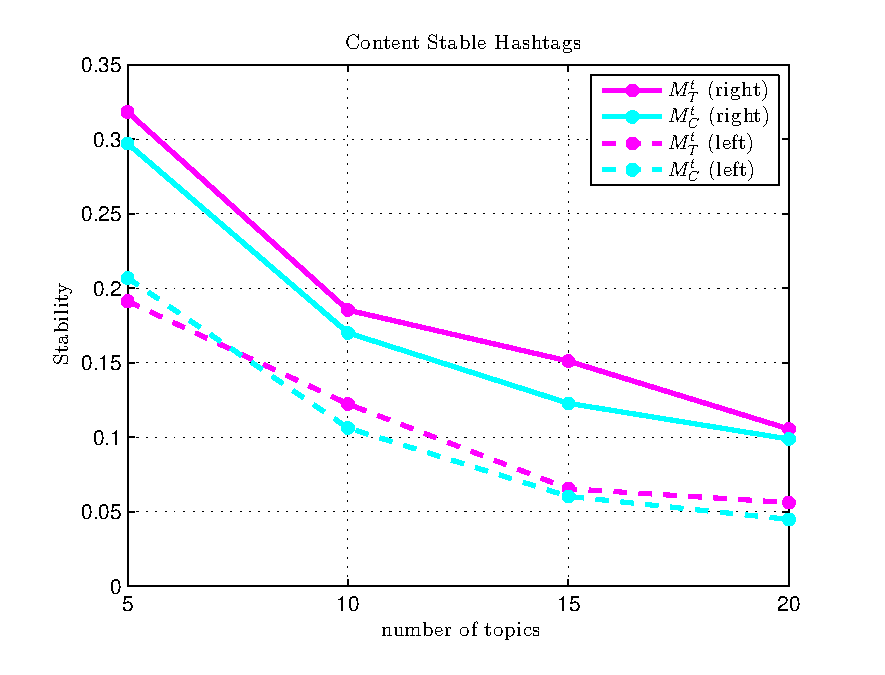
\includegraphics[width=\textwidth]{KDD/images/content_stable_eigen_left_right}          
	%{\tiny(a) Content Stable }
\end{minipage} 
\begin{minipage}{0.49\linewidth}
  \centering
  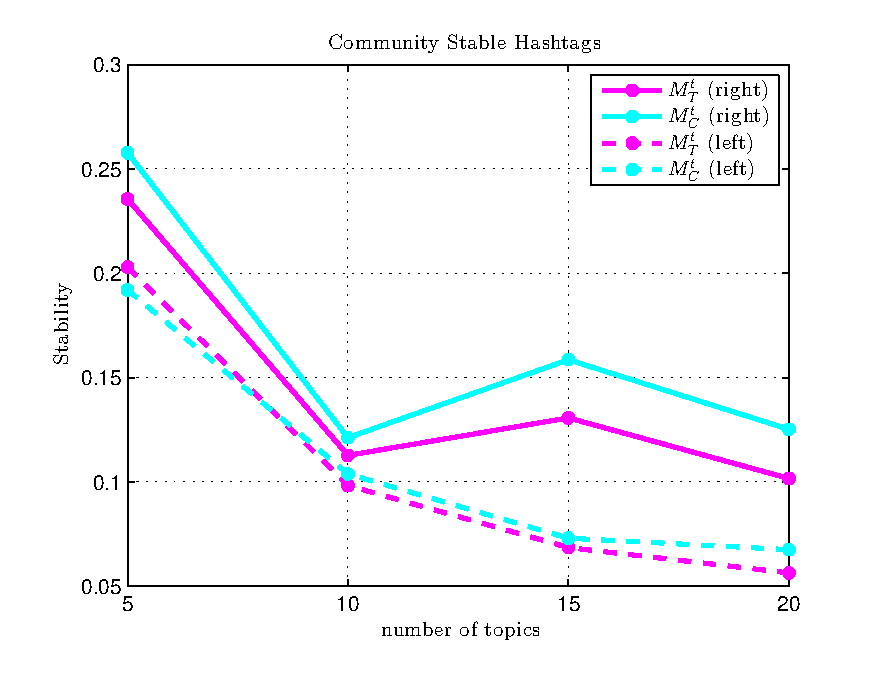
\includegraphics[width=\textwidth]{KDD/images/community_stable_eigen_left_right}             
	%{\tiny(b) Community Stable}
\end{minipage} 
  \caption[Stability of evolution matrices]{{This figure plots the stability of $\MC$ and $\MT$.
We note that in (a) $\MT$ matrix shows higher stability than the $\MC$ matrix,
and in (b) $\MC$ shows higher stability than $\MC$, thus confirming that we are indeed able to learn the 
stability through our algorithm.}}
  \label{fig:stability_analysis}
}
\end{center}
\end{figure*}


% CONCLUSIONS AND FUTURE WORKS.
\vspace{-0.3cm}
\section{Conclusion}
\label{sec:conclusion}
The goal of our work was to gain a better understanding of when social context
helps in modeling topic evolution.  In order to achieve this, we proposed a matrix factorization based
approach which takes into account both the content of the documents and their social
context.  We found that, depending on the kind of topic, there is a clear trade
off between the content and community.
The content of the document
suffices if the text of the topic is very focused, and evolves little over time.
As we begin to move away from this scenario to consider documents that have a richer
and more variable vocabulary, we find that the use of social context
begins to help greatly.  We were also able to show
that our model can learn the kind of topics at hand; i.e., whether they are
content stable, community stable, or
both.

This work predominantly considered the user interactions of the documents
as the social context.  In the same spirit, one could explore what it means to consider
other types of contexts like geographical location of the user (or document),
and also perhaps delve more into the user profiles and incorporate information
about age, gender and demographics to give a well rounded view of the social context.
We hope to be able to work on these aspects in the future.
\section{Acknowledgements}
J.K. and G.R.G.L. acknowledge support from Yahoo! Inc., 
and the NSF (grants CCF-0830535 and IIS-1054960). 
G.R.G.L. acknowledges support from the Alfred P. Sloan Foundation.
D.S is funded by the EC SUPER (FP7-606853) project.
\vspace{-0.2cm}
{\small\bibliographystyle{plain}
\bibliography{refs}}
\end{document}
